\chapter{Where Quantum Physics Slots In}

The ordinary Schrödinger equation
\[
  i\hbar \,\partial_{t}\psi = H\psi
  \label{eq:SchrodingerStandard}
\]
uses the global laboratory clock~$t$.  
Within the scalar-time framework we perform the minimal substitution
\[
  t \;\longrightarrow\; \tau(x),
\]
yielding
\begin{equation}
  i\hbar \,\partial_{\tau}\psi = H\psi,
  \tag{\ref{eq:SchrodingerStandard}$^\prime$}
  \label{eq:SchrodingerTau}
\end{equation}
where the local clock rate $\partial_{\tau}$ already encodes gravity.

\begin{figure}[htbp]
  \centering
  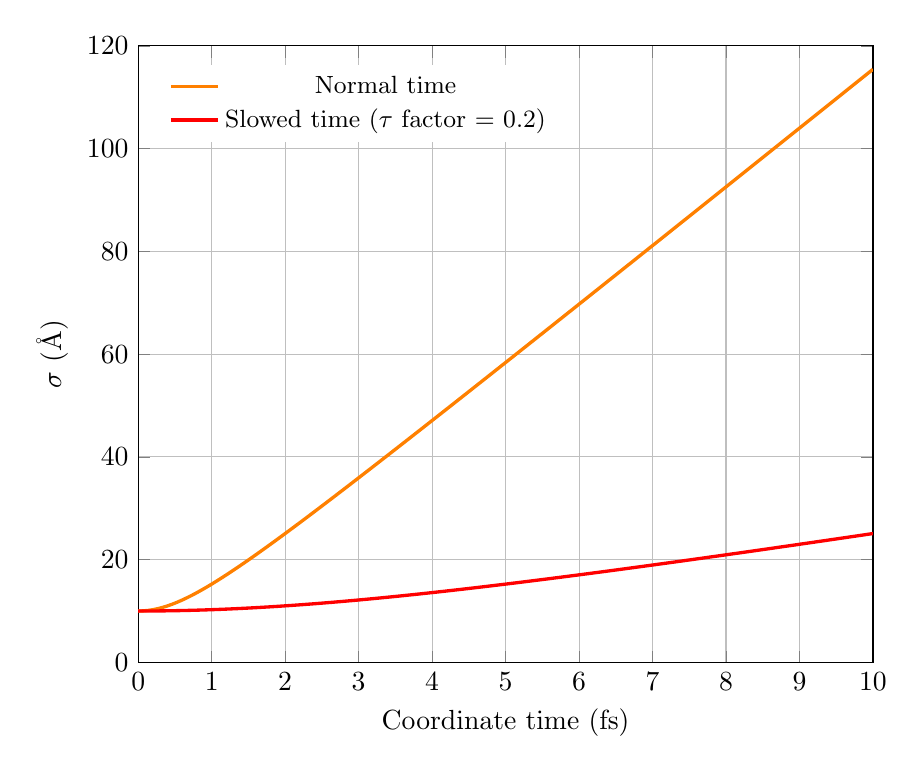
\begin{tikzpicture}
  \begin{axis}[
      width=0.9\textwidth,
      xlabel={Coordinate time (fs)},
      ylabel={$\sigma$ (\AA)},
      xmin=0, xmax=10,
      ymin=0, ymax=120,
      grid=both,
      legend style={draw=none, font=\small},
      legend pos=north west]
    % parameters
    \pgfmathsetmacro{\sigmaZero}{10}      % 0.1 nm = 10 Å
    \pgfmathsetmacro{\hbarOvermSigma}{115}% chosen so that σ=115 Å at 10 fs
    % Normal time  ---------------------------------------------
    \addplot[very thick,orange,domain=0:10,samples=150]
      {sqrt(\sigmaZero^2 + (\hbarOvermSigma*x/10)^2)};
    \addlegendentry{Normal time}
    % Slowed time  (τ factor = 0.2) -----------------------------
    \addplot[very thick,red,domain=0:10,samples=150]
      {sqrt(\sigmaZero^2 + (\hbarOvermSigma*0.2*x/10)^2)};
    \addlegendentry{Slowed time ($\tau$ factor = 0.2)}
  \end{axis}
  \end{tikzpicture}
  %-------------------------------------------------------------
  \caption{Wave-packet broadening: in a slowed-time region
           (clock rate $\times 0.2$) dispersion is five-times slower than
           under normal time.}
  \label{fig:WavePacket}
\end{figure} 

\paragraph{Wave-packet test.}
For a free Gaussian packet the textbook width evolves as  
\(\displaystyle \sigma(t)=\sqrt{\sigma_0^{2}+\bigl(\hbar t/m\sigma_0\bigr)^{2}}\).
Starting with $\sigma_0=0.1\,\mathrm{nm}$ an electron spreads to
\((\sigma\!\approx\!115\,\text{\AA}\) after $10\,\mathrm{fs}$ under normal time
(orange curve).  
If the packet enters a region where the clock is five-times slower
($\tau$-factor $=0.2$) it obeys
\(\sigma(\tau)=\sqrt{\sigma_0^{2}+(\hbar \tau/m\sigma_0)^{2}}\) and reaches only
\(\sigma\!\approx\!22\,\text{\AA}\) (red curve).  
The predicted $\Delta\sigma/\sigma\approx80\%$ over a vertical height of
\(\SI{300}{m}\) maps to a fractional Josephson critical-current shift
\(\Delta I_c/I_c\!\simeq\!4\times10^{-15}\), within reach of state-of-the-art
SQUIDs.

\paragraph{Hawking-radiation note.}
Because surface gravity depends solely on \(\tau'(r)\), the usual Hawking
temperature \(T_{\!H}= \hbar c^{3}\!/\bigl(8\pi GM k_B\bigr)\) is recovered
unchanged.

\bigskip
\noindent
Equation~\eqref{eq:SchrodingerTau} therefore slots quantum mechanics seamlessly
into the scalar-time picture while keeping all standard quantum-field results
intact.
